\documentclass{article}

\usepackage[hidelinks]{hyperref}
%\usepackage[capitalize]{cleveref}
\usepackage{tikz}
\usepackage[all]{xy}
%\usepackage[foot]{amsaddr}
\usepackage{amsmath,amsfonts,amssymb,amsthm}
\usepackage{xcolor}
\usepackage{tabularx}
\usepackage{booktabs}

\newcommand{\SM}[1]{\color{blue}#1\color{black}}
\newcommand{\ZZ}[1]{\color{cyan}#1\color{black}}
\newcommand{\AS}[1]{\color{red}#1\color{black}}

\newcommand{\Q}{\ensuremath{\mathbb Q}}
\newcommand{\Z}{\ensuremath{\mathbb Z}}
\newcommand{\Fp}{\ensuremath{\mathbb F_p}}
\newcommand{\End}{\ensuremath{\text{End}}}

\theoremstyle{definition}
\newtheorem*{remark}{Remark}

\title{Bandersnatch: a fast elliptic curve built over the BLS12-381
  scalar field}
\author{Simon Masson${}^\text{1}$, Antonio Sanso${}^\text{2,3}$ and
  Zhenfei Zhang${}^\text{2}$\\
  \ \\
  ${}^\text{1}$\href{https://anoma.network}{Anoma}\\
  ${}^\text{2}$Ethereum Foundation\\
  ${}^\text{3}$Ruhr Universit{\"a}t Bochum\\
}
\date{}

\makeatletter
\newcommand{\verbatimfont}[1]{\renewcommand{\verbatim@font}{\ttfamily#1}}
\makeatother

\begin{document}

\verbatimfont{\small}%

\maketitle
\medskip
\begin{abstract}
 In this short note, we introduce Bandersnatch, a new elliptic curve
 built over the BLS12-381 scalar field. The curve is equipped with an efficient
 endomorphism, allowing a fast scalar multiplication algorithm.
 Our benchmark shows that the multiplication is 42\% faster, 
 compared to another curve, called Jubjub, having similar
 properties. Nonetheless, Bandersnatch does not provide any
 performance improvement for either rank 1 constraint systems (R1CS)
 or multi scalar multiplications, compared to the Jubjub curve.
\end{abstract}

\section{Introduction}
%BLS12-381
BLS12-381 is a pairing-friendly curve created by Sean
Bowe~\href{https://electriccoin.co/blog/new-snark-curve/}{here} in 2017.
Currently, BLS12-381 is undergoing a standardization process 
from the
IRTF Crypto Forum Research Group, and is
universally used for digital
signatures and zero-knowledge proofs by many projects orbiting in the
blockchain universe: Zcash, Ethereum 2.0, \href{https://anoma.network}{Anoma}, Skale, Algorand, Dfinity,
Chia, and more.
%jubjub
The ZCash team
introduced Jubjub~\href{https://z.cash/technology/jubjub/}{here}, an
elliptic curve built over the BLS12-381 scalar field $\mathbb
F_{r_\text{BLS}}$.
This curve is not pairing-friendly, but leads to constructions where
$\mathbb F_{r_\text{BLS}}$ arithmetic circuits can be manipulated
using the BLS12-381 curve.
The Jubjub curve can be represented in the twisted Edwards
coordinates, allowing efficiency inside zk-SNARK circuits.
In order for some cryptographic applications to scale, it is necessary to
have efficient scalar multiplication on the non-pairing-friendly
curve.
The main drawback of Jubjub is the slow scalar multiplication
algorithm compared, for example, with the ``Bitcoin curve''
(SECP256k1).
It comes from the fact that the curve does not have an efficiently
computable endomorphism, necessary for computing scalar
multiplications using the GLV method~\cite{C:GalLamVan01} (a technique
protected by a US patent until Sep 2020~\cite{glvpatent}, but that 
expired and is
freely usable now).

\paragraph{Our contribution.}
The Jubjub curve is a curve with a large discriminant, meaning that
the GLV method is not possible on this curve.
We performed an exhaustive search of curves of small discriminant,
defined over the BLS12-381 scalar field. This way, we obtain an
elliptic curve using the Complex Multiplication
method~\cite{MC:AtkMor93}, where the scalar multiplication algorithm
is efficient thanks to the GLV method~\cite{C:GalLamVan01}.

We implement this curve in Rust, using
the~\href{http://arkworks.rs}{Arkworks framework}, and release our
code to the open domain~\cite{bandersnatch-rust}.
Table~\ref{tab:comp} shows a comparison of Bandersnatch curve
and Jubjub curve. 
Details deferred to Section~\ref{sec:comparison}.

\begin{table}[ht] %\small
  \centering
  
  \begin{tabular}{|l|c|c|}\hline
      & multiplication cost  \\\hline\hline
    Jubjub & 75 $\mu$s   \\\hline
    Bandersnatch & 44 $\mu$s   \\\hline\hline   
    Improvement & 42\% \\\hline
  \end{tabular}
  \caption{Bandersnatch vs Jubjub}
  \label{tab:comp}
\end{table}

We also report the number of 
% , in terms of both group multiplications and 
% the number of 
constraints one needs to express a group multiplication
in the form of rank one constraint system (R1CS), 
a common approach for expressing circuits for zero-knowledge 
proof systems. 
A group multiplication takes 
3325
constraints when the point is in affine form over the 
twisted Edwards curve.
%, and 
%2361
%constraints when the point is in the projective form
%over the short Weierstrass from.
%Both figures 
This matches what we have for Jubjub curve.

\paragraph{Organization of the paper.}
In Section~\ref{sec:small-disc-curves}, we describe how we obtained
several curves allowing the GLV method together with cryptographic
security.
Then, we introduce in Section~\ref{sec:bandersnatch} the Bandersnatch
curve in different models (in Weierstrass, Montgomery and twisted Edwards
coordinates).
Finally, we compare the scalar multiplication algorithm over
the Bandersnatch and the Jubjub curves in
Section~\ref{sec:comparison} from a practical point of view.


\section{Small discriminant curves}\label{sec:small-disc-curves}

The GLV method~\cite{C:GalLamVan01} is a well known trick for accelerating
scalar multiplication over particular curve. In a nutshell, it applies
to elliptic curves where an endomorphism $\psi$ can be efficiently computed.
The GLV method applies in particular for $j$-invariant $j=0$
(resp. $j=1728$) curves because a non-trivial automorphism can be
computed using only one modular multiplication. % (see Example~\ref{ex:psi-j0}).
The method also applies for other curves where the endomorphism is
slightly more expensive, called \emph{small discriminant} curves.

% notations
Let $E$ be an elliptic curve defined over $\Fp$ of trace $t$. $E$ and
its quadratic twist $E^t$ are $\mathbb F_{p^2}$-isomorphic curves and
their orders over $\Fp$ are closely related with the trace
$t$:
$$\#E(\Fp) = p+1-t\qquad \#E^t(\Fp) = p+1+t.$$
See~\cite{Silverman86} for a complete introduction to elliptic curves.
In this work, we are looking for cryptographic applications based on
ordinary elliptic curves, meaning that we look for $t\not\equiv 0
\bmod p$. The endomorphism ring of these curves have a particular
structure: $\End(E)$ is an order of the imaginary quadratic field
$\Q(\sqrt{t^2-4p})$.
From now, we denote $-D$ to be the discriminant of $\End(E)$, and
$\{\text{Id},\psi\}$ a basis of the endomorphism ring.
The fundamental discriminant corresponds to the discriminant of the
maximal order containing $\End(E)$.
This way, $\psi$ is of degree $\frac{D+1}4$ or $D/4$ depending on the
value of $D$ modulo $4$, and $\psi$ can be defined using polynomials
of degree $O(D)$ thanks to the Vélu's formulas~\cite{velu71}.
Thus, the evaluation of $\psi$ is efficient only for curves of small
discriminant.

In this work, we restrict to curves defined over the BLS12-381 scalar
field $\mathbb F_{r_\text{BLS}}$. From now, we denote $p=r_\text{BLS}$
and we look for curves with a $128$-bit cryptographic security.
Curves with $-D=-3$ and $-4$ do not have a large prime subgroup
defined over $\Fp$.
Hence, we look for small discriminant $-D<-4$ curves with subgroup and
twist-subgroup security. It means that $\#E(\Fp)$ has a roughly 256-bit
prime factor, as well as $\#E^t(\Fp)$.

As the endomorphism cost is closely related to the discriminant, we
restrict to $-D \geq -388$ so that $\psi$ can be efficiently computed.
Moreover, we restrict on fundamental discriminants (discriminants
of the maximal orders of imaginary quadratic fields). We denote
$\mathcal O_{-D}$ the maximal order of discriminant $-D$. Elliptic
curves with $\End(E) \subset \mathcal O_{-D}$ are isogenous curves,
meaning that there is a rational map between them. Isogenous curves
have the same order so that we can restrict on fundamental
discriminants for our search.

We compute an exhaustive search among all the possible (fundamental)
discriminants ($-292 \leq -D \leq -3$).
Given a discriminant $-D$, roughly half of the curves are
supersingular and hence not relevant to our cryptographic
applications.
We list in Table~\ref{tab:group-order-factorization} the ordinary
curves we obtained. In this table, $p_n$ denotes a prime of $n$ bits.
The generation of these curves is reproducible
using~\href{https://github.com/asanso/Bandersnatch/blob/main/python-ref-impl/small-disc-curves.py}{this
  file}.
We finally obtain an interesting curve for $-D = -8$ with large prime
order subgroups on both the curve and its twist.
We present in Section~\ref{sec:bandersnatch} the curve in several
models, together with the endomorphism in order to apply the GLV
scalar multiplication algorithm.

\begin{table*}[!ht]
    \centering\footnotesize
    \begin{tabularx}{\textwidth}{ccl}
        \toprule                            
        $\mathbf{-D}$    & \textbf{Curve sec.}  & \textbf{Curve order} \\
        \midrule        
$-3$ & $65$-bit & $2^{2}  \cdot 3  \cdot 97  \cdot 19829809  \cdot 2514214987  \cdot 423384683867248993  \cdot p_{131}$\\
 & $14$-bit & $2^{64}  \cdot 906349^{4}  \cdot p_{28}^{4}$\\
 & $77$-bit & $7  \cdot 43  \cdot 1993  \cdot 2137  \cdot 43558993  \cdot 69032539613749  \cdot p_{154}$\\
 & $41$-bit & $3  \cdot 7  \cdot 13  \cdot 79  \cdot 2557  \cdot 33811
        \cdot 1645861201  \cdot 75881076241177 \cdot$\\
 &          & $86906511869757553  \cdot p_{82}$\\
 & $13$-bit & $3^{2}  \cdot 11^{2}  \cdot 19^{2}  \cdot 10177^{2}  \cdot 125527^{2}  \cdot 859267^{2}  \cdot 2508409^{2}  \cdot 2529403^{2}  \cdot p_{26}^{2}$\\
 & $118$-bit & $836509  \cdot p_{236}$\\
$-4$ & $59$-bit & $2^{32}  \cdot 5  \cdot 73  \cdot 906349^{2}  \cdot 254760293^{2}  \cdot p_{119}$\\
 & $37$-bit & $2^{2}  \cdot 29  \cdot 233  \cdot 34469  \cdot
        1327789373  \cdot 19609848837063073 \cdot$\\
 &          & $159032890827948314857  \cdot p_{74}$\\
 & $37$-bit & $2  \cdot 3^{2}  \cdot 11^{2}  \cdot 13  \cdot 1481  \cdot 10177^{2}  \cdot 859267^{2}  \cdot 52437899^{2}  \cdot 346160718017  \cdot p_{74}$\\
 & $57$-bit & $2  \cdot 5  \cdot 19^{2}  \cdot 1709  \cdot 125527^{2}  \cdot 2508409^{2}  \cdot 2529403^{2}  \cdot p_{114}$\\
$\mathbf{-8}$ & $\mathbf{122}$\textbf{-bit} & $\mathbf{2^{7}  \cdot 3^{3}  \cdot p_{244}}$\\
 & $\mathbf{126}$\textbf{-bit} & $\mathbf{2^{2}  \cdot p_{253}}$\\
$-11$ & $69$-bit & $5  \cdot 191  \cdot 5581  \cdot 18793  \cdot 48163  \cdot 46253594704380463613  \cdot p_{138}$\\
 & $73$-bit & $3^{3}  \cdot 11^{2}  \cdot 9269797  \cdot 17580060420191283788101  \cdot p_{147}$\\
$-19$ & $110$-bit & $7  \cdot 11^{2}  \cdot 19  \cdot 23  \cdot 397  \cdot 419  \cdot p_{220}$\\
 & $74$-bit & $3^{2}  \cdot 5  \cdot 503  \cdot 10779490483  \cdot 433275286013779991  \cdot p_{149}$\\
$-24$ & $53$-bit & $2^{2}  \cdot 3^{2}  \cdot 7  \cdot 19^{2}  \cdot 127  \cdot 29402034080953  \cdot 2970884754778276642175743  \cdot p_{106}$\\
 & $86$-bit & $2^{5}  \cdot 5  \cdot 39628279  \cdot 1626653036429383  \cdot p_{172}$\\
$-51$ & $112$-bit & $3^{2}  \cdot 5  \cdot 61223923  \cdot p_{224}$\\
 & $120$-bit & $23^{2}  \cdot 41  \cdot p_{241}$\\
$-67$ & $67$-bit & $3479887483  \cdot 56938338857  \cdot 8474085246072233  \cdot p_{135}$\\
 & $79$-bit & $3^{2}  \cdot 8478452882270519617659314063  \cdot p_{159}$\\
$-88$ & $61$-bit & $2^{2}  \cdot 11  \cdot 16984307  \cdot 24567897636186592260640293583411  \cdot p_{122}$\\
 & $66$-bit & $2^{9}  \cdot 3^{2}  \cdot 31  \cdot 6133  \cdot 116471  \cdot 69487476515565975361139  \cdot p_{133}$\\
$-132$ & $73$-bit & $2  \cdot 1753  \cdot 101235113104036296384208928969  \cdot p_{147}$\\
 & $92$-bit & $2  \cdot 3^{2}  \cdot 7^{2}  \cdot 11  \cdot 23  \cdot 587  \cdot 701  \cdot 32299799971  \cdot p_{184}$\\
$-136$ & $62$-bit & $2^{3}  \cdot 7^{3}  \cdot 19^{3}  \cdot 10939  \cdot 11131315086725327441688173207  \cdot p_{125}$\\
 & $87$-bit & $2^{2}  \cdot 5  \cdot 5741  \cdot 30851  \cdot 533874022134253  \cdot p_{175}$\\
$-228$ & $114$-bit & $2  \cdot 3^{2}  \cdot 19  \cdot 89  \cdot 5189  \cdot p_{228}$\\
 & $81$-bit & $2  \cdot 947  \cdot 277603  \cdot 28469787063396608749  \cdot p_{162}$\\
$-244$ & $89$-bit & $2^{2}  \cdot 13  \cdot 523  \cdot 1702319  \cdot 2827715661581  \cdot p_{179}$\\
 & $88$-bit & $2^{8}  \cdot 3^{2}  \cdot 5  \cdot 71  \cdot 907  \cdot 2749  \cdot 146221  \cdot 2246269  \cdot p_{176}$\\
$-264$ & $83$-bit & $2^{3}  \cdot 11  \cdot 131  \cdot 12543757399  \cdot 2818746796297  \cdot p_{167}$\\
 & $82$-bit & $2^{2}  \cdot 3  \cdot 5^{2}  \cdot 2287  \cdot 2134790941497418864559  \cdot p_{165}$\\
$-276$ & $70$-bit & $2  \cdot 11^{2}  \cdot 8839  \cdot 78797899  \cdot 323360863688748558301  \cdot p_{140}$\\
 & $88$-bit & $2  \cdot 3  \cdot 5  \cdot 6197  \cdot 138617  \cdot 16664750312513  \cdot p_{177}$\\
$-292$ & $92$-bit & $2  \cdot 54983  \cdot 5220799  \cdot 2671917733  \cdot p_{185}$\\
 & $86$-bit & $2  \cdot 11^{2}  \cdot 149  \cdot 354689  \cdot
24012883  \cdot 32483123  \cdot p_{172}$\\
\bottomrule
    \end{tabularx}
    \caption{Curves for discriminants $-3 \geq -D \geq -292$.}
    \label{tab:group-order-factorization}
\end{table*}

\section{Bandersnatch}\label{sec:bandersnatch}

The Bandersnatch is obtained from a discriminant $-D = -8$, meaning
that the endomorphism ring is $\Z[\sqrt{-2}]$.
We obtain the curve $j$-invariant using the Complex Multiplication
method, based on the Hilbert class polynomial $H_{-D}(X)$.
The roots of $H_{-D}$ are $j$-invariants of elliptic curves whose
endomorphism ring is of discriminant $-D$.
From a $j$-invariant, we obtain the curve equation in different
models. Before looking into the details of three different representations,
we briefly recall how to exhibit the degree $2$ endomorphism $\psi$.

\paragraph{Degree 2 endomorphism.}
The endomorphism $\psi$ has a kernel generated by a $2$-torsion
point. Hence, we can obtain the rational maps defining $\psi$ by
looking at the curves $2$-isogenous to Bandersnatch. Only one has the
same $j$-invariant, meaning that up to an isomorphism, the Vélu's
formulas~\cite{velu71} let us obtain compute $\psi$.
For cryptographic use-cases, we are interested in computing $\psi$ on
the $p_{253}$-order subgroup of the curve. On these points, $\psi$
acts as a scalar multiplication by the eigenvalue
$$\lambda = \text{\small{\tt
    0x13b4f3dc4a39a493edf849562b38c72bcfc49db970a5056ed13d21408783df05}}.$$
By construction, $\psi$ is the endomorphism $\sqrt{-2}\in \mathcal
O_{-8}$. Thus, $\lambda$ satisfies
$\lambda^2+2 = 0 \bmod p_{253}$.
In the following sections, we provide details on the curve equation,
the $\psi$ rational maps, and a generator of the $p_{253}$-order
subgroup in the case of the affine Weierstrass, projective Montgomery
and projective twisted Edwards representations.
The parameters are reproducible using the script
of~\href{https://github.com/asanso/Bandersnatch/blob/main/python-ref-impl/get\_params.py}{this
  file}.

\subsection{Weierstrass curve}\label{sec-w-curve}
\paragraph{Curve equation.}
The Bandersnatch curve can be represented in the Weierstrass model
using the equation
$$E_W:y^2 = x^3 -3763200000x -78675968000000.$$
%% \begin{verbatim}
%% p=0x73eda753299d7d483339d80809a1d80553bda402fffe5bfeffffffff00000001
%% E=EllipticCurve(GF(p), [-3763200000, -78675968000000])
%% \end{verbatim}

\paragraph{Endomorphism.}
The endomorphism $\psi$ can obtained using the method detailed above.
We obtain the following expression:
$$\psi_\text{W}(x,y) = \left(u^2\cdot \frac{x^2+44800x+2257920000}{x+44800}, u^3\cdot
y\cdot \frac{x^2+2\cdot 44800x+t_0}{(x+44800)^2}\right).$$
\begin{verbatim}
u=0x23c58c92306dbb96236140669daf1e2420ffd8fc8de2036c69307ddaa306c7d4
t0=0x73eda753299d7d483339d80809a1d80553bda402fffe5bfefffffffef10be001.
\end{verbatim}

\paragraph{Subgroup generator.}
The generator of the $p_{253}$-order subgroup is computed by finding the
lexicographically smallest valid $x$-coordinate of a point of the
curve, and scaling it by the cofactor $4$ such that the result is not
the point at infinity. From a point with $x=2$, we obtain a generator $E_W(x_W,y_W)$ where:
$$x_W = \text{{\small{\tt 0xa76451786f95a802c0982bbd0abd68e41b92adc86c8859b4f44679b21658710,}}}$$
$$y_W = \text{{\small{\tt 0x44d150c8b4bd14f79720d021a839e7b7eb4ee43844b30243126a72ac2375490a.
}}}$$


\subsection{Twisted Edwards curve}
\paragraph{Curve equation.}
Bandersnatch can also be represented in twisted Edwards coordinates,
where the group law is complete.
In this model, the Bandersnatch curve can be defined by the equation
$$E_\text{TE}:-5x^2+y^2 = 1 +
dx^2y^2, d=\frac{138827208126141220649022263972958607803}{171449701953573178309673572579671231137}.$$
Twisted Edwards group law is more efficient with a coefficient
$a = -1$ (see~\cite{AC:HWCD08} for details).
In our case, $-5$ is not a square in $\Fp$. Thus, the curve with
equation $-x^2+y^2 = 1 -dx^2y^2/5$ is the quadratic twist of
Bandersnatch. We provide a representation with $a=-5$, leading to a
slightly more expensive group law because multiplying by $-5$ is more
expensive than a multiplication by $-1$, but this cost will be
neglected compared to the improvement of the GLV method. See
Section~\ref{sec:comparison} for details.

\paragraph{Endomorphism.}
From this representation, we exhibit the degree $2$ endomorphism in
twisted Edwards coordinates:
$$\psi_\text{TE}(x,y,z) = (xa_1(y+a_2z)(y+a_3z), b_1(y+b_2z)(y+b_3z)yz^2,
(y+c_1z)(y+c_2z)yz^2)$$
\begin{verbatim}
a1=0x23c58c92306dbb95960f739827ac195334fcd8fa17df036c692f7ddaa306c7d4
a2=0x52c9f28b828426a561f00d3a63511a882ea712770d9af4d6ee0f014d172510b4
a3=0x2123b4c7a71956a2d149cacda650bd7d2516918bf263672811f0feb1e8daef4d
b1=0x52c9f28b828426a561f00d3a63511a882ea712770d9af4d6ee0f014d172510b4
b2=0x50d06958b6e8ce1ab1b2745bd377e5bde07e867f02611eae1c098cd1519b574a
b3=0x231d3dfa72b4af2d818763ac3629f247733f1d83fd9d3d50e3f6732dae64a8b7
c1=0x5ede5fd005b839be71b70d491ebfddeff693de40b4c002a7fc1ae7171cc9f7b5
c2=0x150f478323e54389c182cabeeae1fa155d29c5c24b3e595703e518e7e336084c.
\end{verbatim}
This map can be computed in 17 multiplications and 6 additions modulo $p$.

\paragraph{Subgroup generator.}
The generator of the $p_{253}$-order subgroup obtained in
Section~\ref{sec-w-curve} has twisted coordinates
of the form $E_\text{TE}(x_\text{TE},y_\text{TE},1)$ with
$$x_{TE} = \text{{\small{\tt 0x29c132cc2c0b34c5743711777bbe42f32b79c022ad998465e1e71866a252ae18,}}}$$
$$y_{TE} = \text{{\small{\tt 0x2a6c669eda123e0f157d8b50badcd586358cad81eee464605e3167b6cc974166.
}}}$$


\subsection{Montgomery curve}
\paragraph{Curve equation.}
A twisted Edwards curve is always birationally equivalent to a
Montgomery curve. We obtain the mapping between these two
representations following~\cite{JCEng:CosSmi18}.
While the twisted Edwards model fits better for $\mathbb F_p$ circuit
arithmetic and more generally for the zero-knowledge proof context, we
provide here the Montgomery version because the scalar multiplication
is more efficient in this model:
$$E_M: By^2 = x^3 + Ax^2 + x$$
\begin{verbatim}
B=0x300c3385d13bedb7c9e229e185c4ce8b1dd3b71366bb97c30855c0aa41d62727
A=0x4247698f4e32ad45a293959b4ca17afa4a2d2317e4c6ce5023e1fd63d1b5de98.
\end{verbatim}

\paragraph{Endomorphism.}
Montgomery curves allow efficient scalar multiplication using the
Montgomery ladder. We provide here the endomorphism $\psi$ in this
model:
$$\psi_\text{M}(x,-,z) = (-(x-z)^2 - cxz, -, 2xz)$$
\begin{verbatim}
c=0x4247698f4e32ad45a293959b4ca17afa4a2d2317e4c6ce5023e1fd63d1b5de9a.
\end{verbatim}

\paragraph{Subgroup generator.}
The generator of the $p_{253}$-order subgroup given above is of the
form $E_M(x_M,-,1)$ with:
\begin{verbatim}
                xM = 0x67c5b5fed18254e8acb66c1e38f33ee0
                       975ae6876f9c5266a883f4604024b3b8.
\end{verbatim}


\subsection{Security of Bandersnatch}

The Bandersnatch curve order is $2^2\cdot r$ for a $253$-bit long
prime $r$.
% 13108968793781547619861935127046491459309155893440570251786403306729687672801
Its quadratic twist has order
$2^7 \cdot 3^3 \cdot r'$, where $r'$ is another prime of $244$ bits.
%15172417585395309745210573063711216967055694857434315578142854216712503379
Hence, the Bandersnatch curve satisfies twist security after a quick cofactor
check.
We estimate that the Bandersnatch curve (resp. its quadratic twist)
has $126$ bits of security (resp. $122$ bits of security).

% \ZZ{TODOs: 1. expand the security section 2. hash to curve (not essential, but nice to have)
% 3. serialization (required by a spec rather than an academic paper. may be borrow 
% some ed25519 trick where the cofactor is 8?)}

\section{Comparison}\label{sec:comparison}

%### Scalar multiplication improvement
The twisted Edwards representation is mostly used in practice, and we
now focus on the comparison between Jubjub and Bandersnatch in this
model.

\subsection{Scalar multiplications for a variable base point}
% Jubjub scalar multiplication
Because of its large discriminant, the scalar multiplication on Jubjub
is a basic double-and-add algorithm, meaning that it computes a
multiplication by $n$ in $\log n$ doublings and $\log n/2$
additions (in average) on the curve. 

% Bandersnatch scalar multiplication
The endomorphism $\psi$ lets us compute the scalar multiplication
faster than a double-and-add algorithm with few precomputations. For a
point $P$ and a scalar $n$, we first evaluate $\psi$ at $P$ and
decompose $n = n_1 + \lambda n_2$. Then a multi scalar multiplication
is computed in $\log n/2$ doublings and $3\log n/8$ additions (in average) on the curve.

% Benchmarks
We benchmarked our implementation with both GLV enabled and disabled, and 
compared it with Arkworks' own Jubjub implementation. 
Our benchmark is conducted over an AMD 5900x CPU, with Ubuntu 20.04,
rust 1.52 stable version, and Arkwork 0.3.0 release version.
We used~\href{https://docs.rs/criterion}{\texttt{criterion}
  micro-benchmark toolchain},  version 0.3.0, for data collection. We
compile Arkworks with two options, namely \texttt{default} and
\texttt{asm}, respectively.
The \texttt{default} setup relies on \texttt{num\_bigint} crate for
large integer arithmetics, while \texttt{asm} turns on assembly for
finite field multiplication. 

Arkworks use the aforementioned double-and-add
multiplication methodology, without side channel protections such 
as Montgomery ladders. Our non-GLV implementation also follows
this design. For our GLV implementation, there are three components,
namely, the endomorphism, the scalar decomposition, and the
multi scalar multiplication (MSM). We implement those schemes and 
present the micro-benchmarks in Table~\ref{tab:comp_full}.
Specifically, we do not use the MSM implementation in Arkworks:
our scalars, after the decomposition, contain roughly 128 bits
of leading zeros, and our own MSM implementation is 
optimized for this setting.

Table~\ref{tab:comp_full} presents the full picture of the benchmark.
When GLV is disabled, we observe a similar but a little worse 
performance for Bandersnatch curve, compared to
the Jubjub curve, due to the slightly larger coefficient 
$a=-5$ and a larger scalar field of 253 bits (Jubjub curve has $a=-1$
and a scalar field of 252 bits).
When GLV is enabled, we report a 45\% improvement of the Bandersnatch
curve, and a 42\% improvement over the Jubjub curve.

\begin{table}[ht] %\small
  \centering
  
  \begin{tabular}{|l|c|c|}\hline
      & \texttt{default} & \texttt{asm}\\\hline\hline
    Jubjub & 75 $\mu$s & 69 $\mu$s \\\hline\hline
    Bandersnatch without GLV & 78 $\mu$s & 72 $\mu$s  \\\hline\hline   
    Bandersnatch with GLV& 44 $\mu$s & 42 $\mu$s \\\hline
    \ \ \ Endomorphism & 2.4 $\mu$s& 1.8 $\mu$s\\\hline
    \ \ \ Scalar decomposition & 0.75 $\mu$s & 0.7 $\mu$s \\\hline
    \ \ \ multi scalar multiplication & 42 $\mu$s &  40.8 $\mu$s\\\hline\hline
    Overall Improvement & 42\% & 39\% \\\hline
  \end{tabular}
  \caption{Bandersnatch vs Jubjub: Performance}
  \label{tab:comp_full}
\end{table}

To make a meaningful comparison, we benchmark
the cost of the group multiplication over the default generators.
Note that Arkworks do not implement optimizations for 
fixed generators nonetheless. We then sample field elements 
uniformly at random, for each new iteration, and the benchmark
result is consolidated over 100 iterations.

\subsection{Multi scalar multiplications}
This section reports the performance of variable base 
multi scalar multiplications (MSM). Note that this MSM is 
compatible, but
different
from the MSM inside the GLV. 
In particular, for a sum of $k$ scalar multiplications,
we report the data point for: 
\begin{itemize}
  \item invoking the MSM over the $k$ base scalars randomly sampled,
    expected to be around 256 bits;
  \item using GLV endomorphism to break the $k$ base scalars into $2k$
    new base scalars, of halved size, i.e.~of 128 bits.
\end{itemize}
The data is presented in Figure~\ref{fig:msm}. Specifically, 
as a baseline, the trivial solution, captained by 
{\em GLV without 
MSM}, is the product of the number of bases and the cost of
doing a single GLV multiplication. 
Note that the MSM algorithms incur an overhead to build some
tables, which make them less favorable compared to the trivial
solution when dimension is really small. For a dimension greater 
than 4, MSM algorithms begin to out-perform trivial solutions.
For dimension greater than 128, it is more efficient to 
invoke the MSM directly, rather than doing it over the GLV basis.
The reason is that the size of the basis becomes too large, so
that the gain we get from halving the scalars is offset from the
gain we get from halving the basis. We remark that this threshold
point is platform dependent.
\begin{figure}[h]\centering \label{fig:msm}
  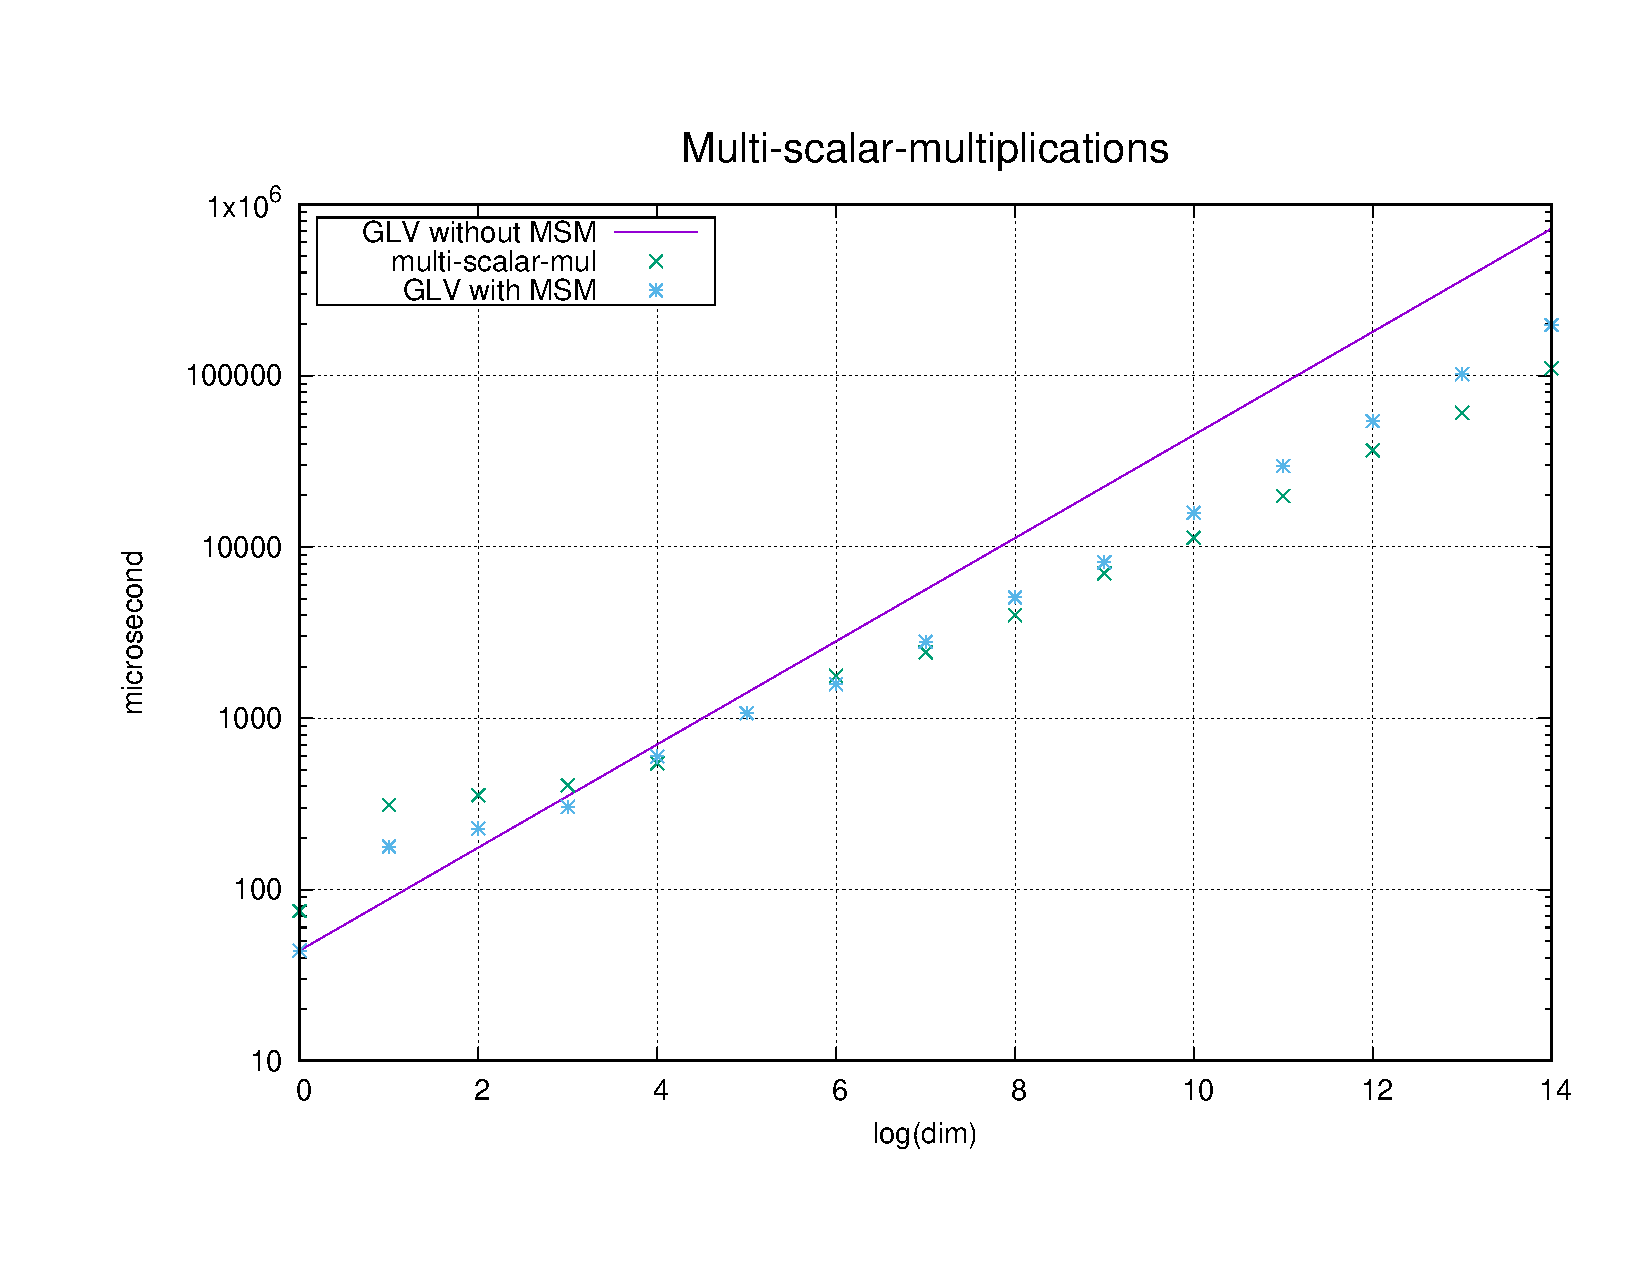
\includegraphics[width=12cm]{fig/msm.pdf}
\end{figure}

\subsection{R1CS constraints}
The Bandersnatch curve is zk-SNARK friendly: its 
base field matches the scalar field for the BLS12-381 curve, a 
pairing-friendly curve, on top of which people build zk-SNARK
systems, such as Groth16 \cite{EC:Groth16} or Plonk \cite{EPRINT:GabWilCio19}.
In such a setting, the prover can sufficiently argue certain 
relationships over arithmetic circuits rather than binary
circuits.
The circuit is expressed in a form of Rank-1 constraint system
(R1CS), and in general, the complexity is determined by the 
number of constraints in an R1CS. 

We evaluate the number of constraints for a 
variable base group multiplication. For a double-and-add
algorithm, 
our code reports 3325 constraints in 
total.
As a sanity check, within the core logic,
it takes 6 constraints per addition, 5 constraints
per doubling and 2 constraints per bit selection. This adds
up to 13 constraints per bit, or 3315 constraints per
group multiplication (and we reasonably assume some system overhead
consumes another 10 constraints). 

% Now, in the case of GLV,
% % Let us first explain the obstacle of implementing the GLV
% %with R1CS. T
% the endomorphism is almost free: it requires 
% 10 constraints. The MSM inside the GLV can also be done 
% with some $2200$ constraints using the above  double-then-add
% techniques.
% The difficult part is the circuit for scalar decomposition,
% which is to prove $n = n_1 +\lambda n_2 \bmod r$ where
% $n$ and $\lambda$ are around 256 bits,
% $n_1$ and $n_2$ are around 128 bits, and
% $r$
% is the order of the scalar field.
% It was estimated that this would add another $300$ constraints
% with hand optimization \cite{daira_telegram}. 

%On the other hand, we can indeed perform a group operation
%over short Weierstrass form with 2361 constraints.
% (TBD: need to check with Arkworks people on this)

% We therefore report the number of constraints to perform
% a group operation on both Jubjub curve and Bandersnatch 
% curve. We observe that it takes 3325 constraints for the 
% Jubjub curve, for which the statement is argued over 
% the Edwards affine form coordinates. 
% It also takes a same number of constraints
% for Bandersnatch when its coordinates are in this form. 
% However, the Bandersnatch curve also supports a 
% short Weierstrass form, for which we can argue the 
% relationship over the projective coordinates.
% This effectively reduces the number of constraints to
% 2361, or a 39\% improvement, as shown in Table~\ref{tab:comp}.
% Note that Jubjub also has a Weierstrass form, but it is 
% not as useful. 
  
% We also want to remark the obstacle of expressing the 
% GLV algorithm in terms of R1CS circuit. We observe a cost of 10 
% constraints for computing the endomorphism, and a cost of 2144 
% constraints for multiple scalar multiplications where the 
% scalars are already decomposed. The cost of those two subroutines
%  is already close
% to the cost of a non-GLV circuit over the projective 
% coordinates. In addition to that, the biggest cost that 
% GLV incurs is to argue the correctness of the scalar 
% decomposition, i.e.~for a scalar $s$, we need to argue 
% that $s = k_1 + k_2 \lambda$ over the scalar field of the
% Bandersnatch curve, 
% for some fixed $\lambda$. To date, we do not have an 
% efficient way for such a proof. The best methods known to us are
% either to argue this relationship bit by bit which incurs a
% prohibitive cost, or to 
% embed the scalars into group elements and argue the relationship
% over the group elements, whose cost will far exceed a 
% single group operation.


% When GLV is enabled, this will be reduced to 1468.
% Precisely, we list the breakdown numbers in Table~\ref{tab:r1cs_full};

% \begin{table}[h] %\small
%   \centering
  
%   \begin{tabular}{|l|c|}\hline
%       & \texttt{default} \\\hline\hline
%       jubjub& 3325 \\\hline
%       Bandersnatch without GLV& 3325 \\\hline\hline
%     Endomorphism & 10 \\\hline
%     Scalar decomposition &  \\\hline
%     multi scalar multiplication & 2144 \\\hline
%     Bandersnatch with GLV&  \\\hline\hline
%     Overall Improvement & \%   \\\hline
%   \end{tabular}
%   \caption{Bandersnatch vs Jubjub: R1CS}
%   \label{tab:r1cs_full}
% \end{table}



%The \href{https://github.com/zhenfeizhang/bandersnatch-glv}{Rust implementation} of the Bandersnatch scalar multiplication
%algorithm confirms our estimations: the GLV method is $40\%$ faster
%than the Jubjub implementation.

\section{Conclusion}
Tne last decade has seen great improvements on practical zk-SNARK systems.
An essential stepping stone of these schemes is an efficient elliptic
curve whose base field matches the scalar field for some pairing-friendly curve.
On this note, we present Bandersnatch as an alternative to the commonly used
base curve Jubjub. Due to the existence of an efficiently computable
endomorphism, the scalar multiplication over this curve is 42\% times
faster than the Jubjub curve.
For multi scalar multiplications, we report a narrowed advantage over Jubjub 
curve when the dimension is small, but it vanishes for larger
dimensions.
We also do not observe any improvement in terms of number of constraints in 
the corresponding R1CS circuit.


\bigskip
\paragraph*{\textbf{Acknowledgments.}} We would like to thank Weikeng Chen, Luca De
Feo, Justin Drake, Dankrad Feist, Gottfried Herold and Daira Hopwood for
fruitful discussions.

\bibliography{bandersnatch,cryptobib/abbrev3,cryptobib/crypto}
\bibliographystyle{unsrt}
\end{document}
